\documentclass[12pt,a4paper]{scrreprt}
%\documentclass[12pt,a4paper,draft,numbers=enddot]{scrreprt}
\linespread{1.25}
%\RedeclareSectionCommand[beforeskip=2cm]{chapter}
\RedeclareSectionCommand[beforeskip=5ex, afterskip=1ex]{section}
\RedeclareSectionCommand[beforeskip=1ex, afterskip=1ex]{subsubsection}
% New type of section
\newcommand\itemsection[1]{\subsubsection*{#1}}
\newcommand\itemtitle[1]{\textbf{#1}\newline}
% Add dots after section numbers
%\usepackage{secdot}
%\sectiondot{chapter}
%\sectiondot{section}
%\sectiondot{subsection}

% General document formatting
\usepackage[margin=2cm,top=1.1cm,bottom=1cm,includeheadfoot]{geometry}
\usepackage[parfill]{parskip}
\usepackage[utf8]{inputenc}
    
% Related to math
\usepackage{amsmath,amssymb,amsfonts,amsthm}

% Graphics
\usepackage{graphicx}

% Preventing hyphenation
%\usepackage[none]{hyphenat}

% Colors
\usepackage{xcolor}
\definecolor{bgr}{HTML}{f9f9f9}
\definecolor{blue}{HTML}{0d8bcf}

% Enumerating, itemizing
\usepackage{enumitem}
\setlist[itemize,1]{leftmargin=3ex,topsep=0.0ex,itemsep=0.5ex,label=\textbullet}
\setlist[itemize,2]{leftmargin=4ex,topsep=1.0ex,itemsep=0.5ex,label=$\circ$}

% Coloured boxes
\usepackage[most]{tcolorbox}
\newenvironment{boxitemize}{
	\begin{itemize}}{\end{itemize}
	}
\tcolorboxenvironment{boxitemize}{
	colback=black!4,
	colframe=black!20,
	arc=2pt,
	boxrule=0.5pt,
	boxsep=0em,
	before skip=6pt,
	after skip=6pt
	}
\newtcbox\textmn{
	before upper=\strut,
	verbatim,
	on line,
	size=small,
	top=-0.7ex,
	bottom=-0.7ex,
	left=0.6ex,
	right=0.6ex,
	colframe=black!20,
	colback=black!4
	}
\newtcbox\texttab{
	before upper=\strut,
	on line,
	size=small,
	top=-0.7ex,
	bottom=-0.7ex,
	left=2.0ex,
	right=2.0ex,
	arc=0pt,
	%colframe=blue,
	%colback=blue,
	%colupper=white,
	colframe=black!20,
	colback=black!4
	}

\newcommand\image[1]{
	\tcbincludegraphics[
		width=\textwidth,
		top=0ex,
		bottom=0ex,
		left=0ex,
		right=0ex,
		boxsep=0em,
		boxrule=0.5pt,
		arc=2pt,
		colframe=black!20
		]
	{#1}
	}
\newcommand\imagenoframe[1]{
	\tcbincludegraphics[
		width=\textwidth,
		top=0ex,
		bottom=0ex,
		left=0ex,
		right=0ex,
		boxsep=0em,
		frame hidden,
		opacityback=0.0
		]
	{#1}
	}


% Font: Computer Modern Sans Serif with Sansmathfonts
%\usepackage{fontawesome}
\usepackage{sansmathfonts}
\usepackage[T1]{fontenc}
\renewcommand*\familydefault{\sfdefault} % Only if the base font of the document is to be sans serif
%\usepackage{microtype}
\usepackage[english]{babel}


% Page headers and footers
\usepackage{fancyhdr}
\pagestyle{fancy}
\fancyhead[LE,RO]{}%{\rightmark}
\fancyhead[LO,RE]{\nouppercase{\leftmark}}
\fancyfoot[C]{\thepage}


% Hyperlinks
\usepackage{hyperref}
\hypersetup{
    bookmarks=true,         % show bookmarks bar?
    unicode=false,          % non-Latin characters in Acrobat’s bookmarks
    pdftoolbar=true,        % show Acrobat’s toolbar?
    pdfmenubar=true,        % show Acrobat’s menu?
    pdffitwindow=false,     % window fit to page when opened
    pdfstartview={FitH},    % fits the width of the page to the window
    pdftitle={My title},    % title
    pdfauthor={Author},     % author
    pdfsubject={Subject},   % subject of the document
    pdfcreator={Creator},   % creator of the document
    pdfproducer={Producer}, % producer of the document
    pdfnewwindow=true,      % links in new PDF window
    colorlinks=true,        % false: boxed links; true: colored links
    linkcolor=blue,         % color of internal links (change box color with linkbordercolor)
    citecolor=blue,         % color of links to bibliography
    filecolor=blue,         % color of file links
    urlcolor=blue,          % color of external links
}
\urlstyle{sf}

% TOC settings
%\setcounter{tocdepth}{1} % Show sections
%\setcounter{tocdepth}{2} % + subsections
%\setcounter{tocdepth}{3} % + subsubsections
%\setcounter{tocdepth}{4} % + paragraphs
%\setcounter{tocdepth}{5} % + subparagraphs

% Begin
\begin{document}
\pagenumbering{roman} % Start roman numbering

% Cover page
\pagecolor{bgr}
\begin{titlepage}

\newcommand\tspace{\vspace*{1.7em}}

\centering

\tspace


\includegraphics[width=0.5\textwidth]{images/davinci-logo.pdf}

{\Large User Manual (3 Apr 2018)\par}

\tspace

{\LARGE A Scientific Software for the Visualization and\\ Processing of Single-Crystal Diffraction Data\\ Measured with a Point Detector\par}

\tspace

{\Large Andrew Sazonov\par}
{\Large \url{http://davinci.sazonov.org}}

\tspace

\hspace*{-2cm}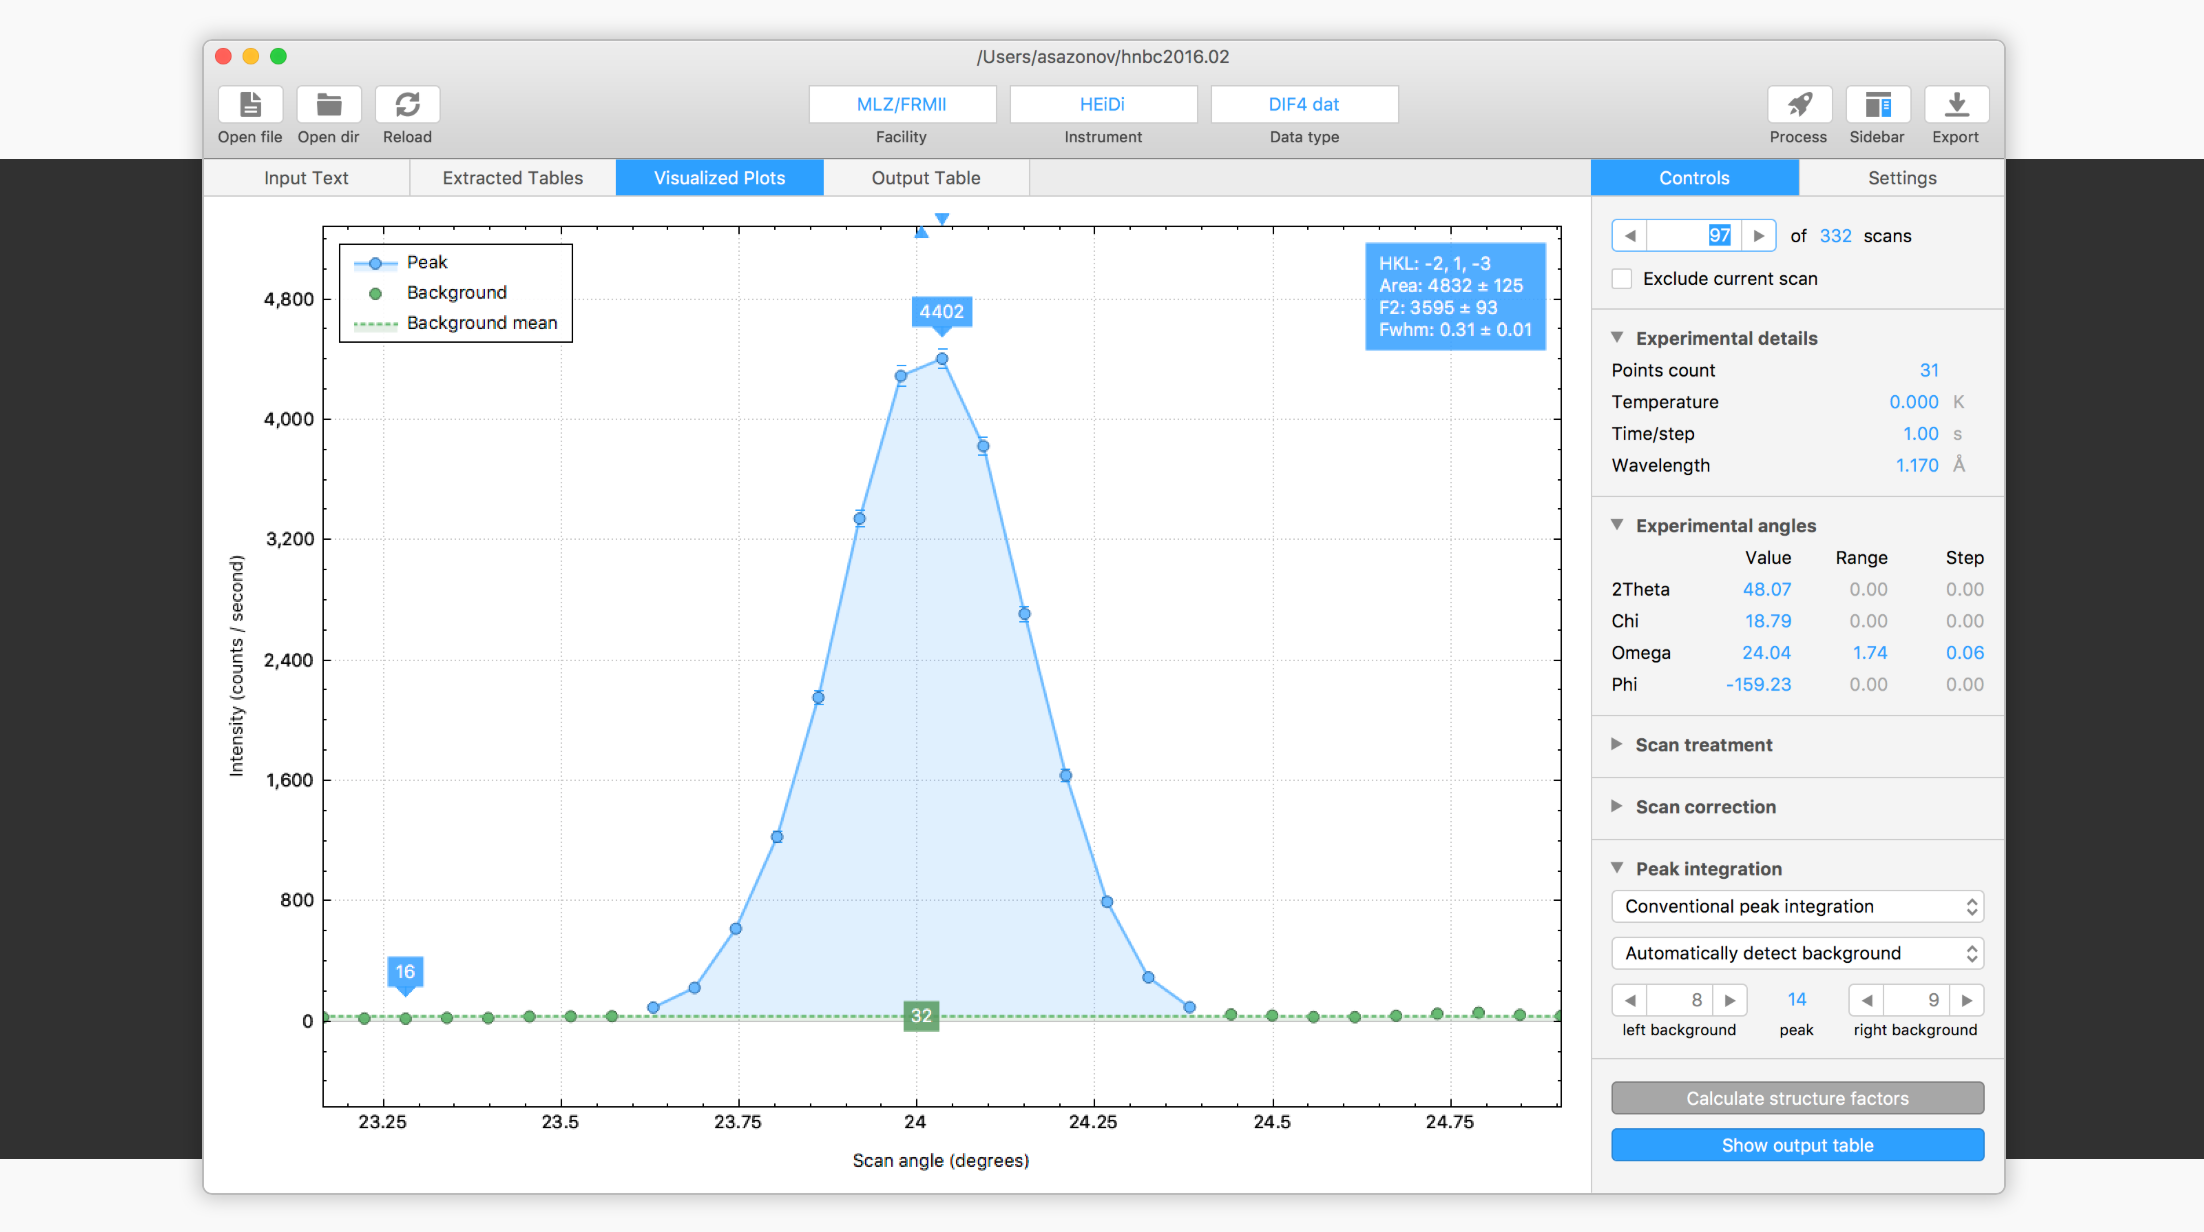
\includegraphics[width=\paperwidth]{images/cover_image.png}

\vfill

\end{titlepage}
\pagecolor{white}






% Create table-of-content
\tableofcontents
\newpage
\pagenumbering{arabic} % Switch to normal numbers

% Input chapters from separate files
\chapter{Introduction}

\textbf{Davinci} is a free scientific software for the visualization and processing of single-crystal diffraction data measured with a point detector.

%===========================================================
\section{What Is Davinci For?}
%===========================================================

\textbf{Davinci} allows to obtain the squares of the structure factors (\(F^2_\text{obs}\)) based on the calculation of integrated intensities of the measured Bragg peaks. \(F^2_\text{obs}\) are required for structure determination with the crystallographic software \textbf{FullProf}, \textbf{Jana2006}, \textbf{ShelX}, etc.

%===========================================================
\section{Davinci Features}
%===========================================================

\begin{itemize}
	\item \textbf{Cross-platform}\\	
	Davinci works across operating systems. You can download precompiled binaries of \textbf{Davinci Installer} for \textbf{macOS}, \textbf{Windows} and \textbf{Linux} operating systems, or you can get the source code and build the program yourself.
	\item \textbf{Easy to use}\\
	Intuitive tabbed interface helps to speed up the treatment of the complete dataset or individual peaks.
	\item \textbf{Various supported instruments}\\
	Davinci accepts the data from \textbf{POLI}, \textbf{HEiDi} and \textbf{MIRA} at \textbf{MLZ} as well as \textbf{6T2} at \textbf{LLB} and \textbf{TriCS} at \textbf{SINQ}.
	\item \textbf{Different peak integrations}\\
	The conventional and Lehmann-Larsen algorithms for the definition of the peak and background parameters.
	\item \textbf{Build-in text editor}\\
	Simplify the analysis of the experimental log and data files.
	\item \textbf{Multiple output formats}\\
	Davinci allows to save the modified input file (txt), extracted peak plots (jpg, pdf) as well as the hkl table (txt).
\end{itemize}
\chapter{Getting Started}

This chapter is about getting started with \textbf{Davinci}.

%===========================================================
\section{Installing and Launching Davinci}
%===========================================================

Davinci works across operating systems. You can download precompiled binaries of \textbf{Davinci Installer} for \textbf{macOS}, \textbf{Windows} and \textbf{Linux} operating systems, or you can get the source code and build the program yourself.

%-----------------------------------------------------------
\subsubsection{Windows}
%-----------------------------------------------------------

\begin{itemize}
	\item Visit the \href{http://davinci.sazonov.org/}{Davinci download page.}
	\item Choose \textbf{Download for Windows.}
	\item Unzip the downloaded \textbf{DavinciInstaller} zip file.
	\item Double-click \textbf{DavinciInstaller.exe} and follow the instructions given by the installer.
\end{itemize}

%-----------------------------------------------------------
\subsubsection{macOS}
%-----------------------------------------------------------

\begin{itemize}
	\item Visit the \href{http://davinci.sazonov.org/}{Davinci download page.}
	\item Choose \textbf{Download for macOS}.
	\item Unzip the downloaded \textbf{DavinciInstaller} zip file.
	\item Click \textbf{DavinciInstaller.app} and follow the instructions given by the installer.
	\item If you see the message \textit{``DavinciInstaller.app can't be opened because it is from an unidentified developer''}, do the following:
	\begin{itemize}
		\item In the \textbf{Finder}, locate the \textbf{DavinciInstaller.app}
		\item Control-click the app icon, then choose Open from the shortcut menu.
		\item Click Open.
		\item The app is saved as an exception to your security settings, and you can open it in the future by double-clicking it just as you can any registered app. More details at \url{https://support.apple.com/kb/PH25088}
  \end{itemize}
\end{itemize}

%-----------------------------------------------------------
\subsubsection{Linux}
%-----------------------------------------------------------

\begin{itemize}
	\item Visit the \href{http://davinci.sazonov.org/}{Davinci download page.}
	\item Choose \textbf{Download for Linux}.
	\item Unzip the downloaded \textbf{DavinciInstaller} zip file.
	\item Double-click \textbf{DavinciInstaller} and follow the instructions given by the installer.
\end{itemize}

%===========================================================
\section{Launching Davinci from the command line}
%===========================================================

The Davinci package provides also the separate command-line version \textbf{DavinciConsole}, which uses the same libraries as \textbf{Davinci}. You can run \textbf{DavinciConsole} from the terminal with the \texttt{-h} or \texttt{--help} flags to get help text with all the available options.

%===========================================================
\section{Updating Davinci}
%===========================================================

\textbf{Davinci} can automatically check for updates every time the program is started. You can always change this setting in the program preferences. You can also manually check for updates.

%-----------------------------------------------------------
\subsubsection{Windows}
%-----------------------------------------------------------

\subparagraph{Check automatically}

\begin{itemize}
	\item In the \textbf{Help} menu, click \textbf{Preferences}.
	\item In the \textbf{Update} group, click \textbf{Automatically check for updates}.
\end{itemize}

\subparagraph{Check manually}

\begin{itemize}
	\item In the \textbf{Help} menu, click \textbf{Check for Updates}.
\end{itemize}

%-----------------------------------------------------------
\subsubsection{macOS}
%-----------------------------------------------------------

\subparagraph{Check automatically}

\begin{itemize}
	\item In the \textbf{Davinci} menu, click \textbf{Preferences}.
	\item In the \textbf{Update} group, click \textbf{Automatically check for updates}.
\end{itemize}

\subparagraph{Check manually}

\begin{itemize}
	\item In the \textbf{Davinci} menu, click \textbf{Check for Updates}.
\end{itemize}

%-----------------------------------------------------------
\subsubsection{Linux}
%-----------------------------------------------------------

\subparagraph{Check automatically}

\begin{itemize}
	\item In the \textbf{File} menu, click \textbf{Preferences}.
	\item In the \textbf{Update} group, click \textbf{Automatically check for updates}.
\end{itemize}

\subparagraph{Check manually}

\begin{itemize}
	\item In the \textbf{Help} menu, click \textbf{Check for Updates}.
\end{itemize}

%===========================================================
\section{Uninstalling Davinci}
%===========================================================

You can uninstall \textbf{Davinci} from \textbf{macOS}, \textbf{Windows} or \textbf{Linux} any time.

%-----------------------------------------------------------
\subsubsection{Windows}
%-----------------------------------------------------------

\begin{itemize}
	\item Open \textbf{Windows Explorer} and navigate to the folder containing installed \textbf{Davinci}.
	\item Double-click \textbf{DavinciUninstaller.exe} and follow the instructions given by the uninstaller.
\end{itemize}

%-----------------------------------------------------------
\subsubsection{macOS}
%-----------------------------------------------------------

\begin{itemize}
	\item Open \textbf{Finder} and navigate to the folder containing installed \textbf{Davinci}.
	\item Click \textbf{DavinciUninstaller.app} and follow the instructions given by the uninstaller.
\end{itemize}

%-----------------------------------------------------------
\subsubsection{Linux}
%-----------------------------------------------------------

\begin{itemize}
	\item Open file manager and navigate to the folder containing installed \textbf{Davinci}.
	\item Click \textbf{DavinciUninstaller} and follow the instructions given by the uninstaller.
\end{itemize}

\chapter{How to Use}

In this chapter we'll look at how to work with \textbf{Davinci}.

%===========================================================
\section{Davinci user interface}
%===========================================================

Here you can see how the program looks like. The application window is divided into parts that provide you with quick and easy access to everything you'll need. The parts are \textbf{Main Window}, \textbf{Sidebar} and \textbf{Toolbar} described in the following sections.

\image{images/ui.png}

%-----------------------------------------------------------
\subsection{Main window}
%-----------------------------------------------------------

The \textbf{Main Window} of the program is located below the \textbf{Toolbar} and it consists of up to 4 tabs, as shown in the figure below. When new files are opened the only first tab is visible. Every next tab appear when the main action on the previous tab is done. You can switch between the available tabs at any time by clicking on their names.

\imagenoframe{images/mainwindow.png}

The following tabs are available and described in the sections below.

\begin{enumerate}
	\item \texttab{Input Text} tab contains the text viewer to show the content of the opened data files.
	\item \texttab{Extracted Tables} tab contains the table viewer to show the data extracted from the opened text files.
	\item \texttab{Visualized Plots} tab contains the graphical viewer to show the plots based on the extracted data.
	\item \texttab{Output Table} tab contains the table viewer with all the calculated parameters for each peak.
\end{enumerate}

%-----------------------------------------------------------
\subsection{Sidebar}
%-----------------------------------------------------------

The application \textbf{Sidebar} is located at right side of the window, below the \textbf{Toolbar}. It has 2 tabs: \texttab{Controls} and \texttab{Settings}. Their contents depend on the selected tab in the \textbf{Main Window}. You can switch between them at any time clicking on the required tab.

\imagenoframe{images/sidebar.png}

\begin{enumerate}
	\item \texttab{Controls} tab provides an access to actions and information fields for the respective data viewer currently selected in the \textbf{Main Window}.
	\item \texttab{Settings} tab provides an access to settings available for the data viewer selected in the \textbf{Main Window}.
\end{enumerate}

The content of the \textbf{Controls} and \textbf{Settings} tabs are described in the sections below individually for every data viewer of the \textbf{Main Window} tabs.

%-----------------------------------------------------------
\newpage
\subsection{Toolbar}
%-----------------------------------------------------------

The toolbar at the top of the window contains the buttons for most important operations as well as some information fields.

\imagenoframe{images/toolbar.png}

The following buttons and information fields are available:

\begin{enumerate}
	\item \textbf{Open file button}: Shows the open file dialog box to select the existing file(s).
	\item \textbf{Open dir button}: Shows the dialog box to open all the files in the existing directory.
	\item \textbf{Reload button}: Reload already opened file(s).
	\item \textbf{Facility information field}: Name of the neutron facility used in the experiment.
	\item \textbf{Instrument information field}: Name of the neutron instrument used in the experiment.
	\item \textbf{Data type information field}: Type of input data.
	\item \textbf{Process button}: Start data processing in auto mode. When the data files are opened, this button allows to go through all the steps in data processing just by single click.
	\item \textbf{Sidebar button}: Show or hide sidebar with options used in the manual data processing.
	\item \textbf{Export button}: Show the save file dialog box to export the document. The available output formats depend on the selected tab in the application \textbf{Main Window}. 
\end{enumerate}

%===========================================================
\newpage
\section{Data processing workflow}
%===========================================================

This section describes all the steps in the manual data processing with \textbf{Davinci}, starting form the opening of input data files and ending with exporting of calculated parameters.

%-----------------------------------------------------------
\subsection{Open files}
%-----------------------------------------------------------

Here you can see how the program looks like when it's just opened.

\image{images/just_opened.png}

You can open selected set of files or all the files in the selected directory in the following different ways:

\begin{itemize}
	\item \textbf{Drag and drop}: By dragging and dropping files or folders onto the main program window.
	\item \textbf{Toolbar buttons}: By clicking the corresponding toolbar buttons and browsing to the desired location.
	\item \textbf{Menu actions}: Via the corresponding \textbf{File} menu actions.
\end{itemize}

%-----------------------------------------------------------
\subsection{Input Text tab}
%-----------------------------------------------------------

When the files are opened, you can see their contents in the text viewer of the \texttab{Input Text} tab. It always shows the content of just single file. You can go through all of them one by one using the \textbf{Go to} spinbox in the \textbf{Sidebar} \texttab{Controls} tab.

\image{images/input_text.png}

The \texttab{Controls} tab of the \texttab{Input Text} allows to:

\begin{itemize}
	\item \textbf{Go to} the specific file among the opened ones by changing the index.
	\item \textbf{Go to} the specific line in the currently shown file.
	\item \textbf{Find} the specific text within the chosen file.
	\item \textbf{Extract data} from all the opened files and switch to the next tab \texttab{Extracted tables}.
\end{itemize}

The \texttab{Settings} tab of the \texttab{Input Text} allows to:

\begin{itemize}
	\item \textbf{Highligh syntax} of the opened text in the text viewer to simplify its reading.
	\item \textbf{Wrap text} lines in the text viewer.
	\item Adjust the text viewer \textbf{Font} family and size according to you personal needs.
\end{itemize}

%-----------------------------------------------------------
\subsection{Extracted Tables tab}
%-----------------------------------------------------------

Here one can see in table view the data extracted from the opened text files. It always shows the single scan data. You can go through all the scans one by one using the \textbf{Go to} spinbox in the \textbf{Sidebar} \texttab{Controls} tab.

\image{images/extracted_tables.png}

The \texttab{Controls} tab of the \texttab{Extracted Tables} allows to:

\begin{itemize}
	\item \textbf{Go to} the specific scan by its index.
	\item \textbf{Exclude current scan} from the data processing and output.
	\item \textbf{Visualize extracted data} in the plot viewer on the next tab \texttab{Visualized Plots}.
\end{itemize}

%-----------------------------------------------------------
\newpage
\subsection{Visualized Plots tab}
%-----------------------------------------------------------

Here one can see the plots based on the extracted data. 

%-----------------------------------------------------------
\subsubsection{Initial visualization}
%-----------------------------------------------------------

As the first step, the untreated data are plotted (in green) as Intensity (counts/second) vs. Scan angle (degrees). If Miller indices $(hkl)$ are available or orientation matrix is given to calculate $(hkl)$, they are shown in the top right angle of the plot. The plot legend is given in the top left angle. The maximum and minimum intensities are indicated on the plot by boxes with arrows. 

\image{images/visualized_plots.png}

The \texttab{Controls} tab of the \texttab{Visualized Plots} allows to:

\begin{itemize}
	\item \textbf{Go to} the specific scan by its index.
	\item \textbf{Exclude current scan} from the data processing and output.
	\item View the \textbf{Experimental details}, such as Date and Time, Temperature, Magnetic Field, Time/step, Wavelength, etc.
	\item View the \textbf{Experimental angles}, the scan ranges and steps during the scan.
	\item \textbf{Calculate structure factors} ($F^2_\text{obs}$) and other parameters, such as full width at half maximum (FWHM), flipping-ratios (FR) if applicable, etc.
\end{itemize}

The \texttab{Settings} tab of the \texttab{Visualized Plots} allows to:

\begin{itemize}
	\item \textbf{Hide legend} in the plot viewer.
\end{itemize}

%-----------------------------------------------------------
\subsubsection{Visualization of the treated data}
%-----------------------------------------------------------

As the second step, the treated data are plotted in the plot viewer. The peak area is shown in blue, while the background in green. The average background intensity is now also indicated on the plot. The calculated peak parameters, such as peak area (Area), structure factor squared (F2), full width at half maximum (FWHM) and others are added in the top right angle of the plot.

\image{images/visualized_plots_calculated.png}

After the peak parameters are calculated, the \texttab{Controls} tab additionally allows to:

\begin{itemize}
	\item Change to the individual treatment of the current scan in \textbf{Scan treatment}.
	\item Apply \textbf{Scan correction}, i.e., to remove the shoulders from the neighbour peaks on the left and/or right side of the scan, if any.
	\item Select \textbf{Peak integration} algorithm and type of the background detection.
	\item \textbf{Show output table} with all the calculated parameters for each peak in the next tab \texttab{Output table}.
\end{itemize}

%-----------------------------------------------------------
\newpage
\subsection{Output Table tab}
%-----------------------------------------------------------

Here one can see the table with all the calculated parameters for each peak.

\image{images/output_table.png}

The \texttab{Controls} tab of the \texttab{Output Table} allows to:

\begin{itemize}
	\item \textbf{Go to} the specific scan by its index.
	\item \textbf{Exclude current scan} from the data processing and output.
	\item \textbf{Export output data} in the different file formats.
\end{itemize}
 
The \texttab{Settings} tab of the \texttab{Output Table} allows to:

\begin{itemize}
	\item \textbf{Export excluded scans} in the output files.
	\item \textbf{Always save headers} in the output files.
\end{itemize}

\newpage
The output table contains all the available parameters. The list of parameters depends on the type of input data. The full list is given below. If the polarized neutron diffraction data are used, additional (+) or (-) suffixes to the parameter names are added, which correspond to two opposite directions of neutron polarisation.
 
\begin{itemize}
	\item \textbf{Excluded}: 1 if peak is excluded or 0 otherwise.
	\item \textbf{Scan}: Index of the scan.
	\item \textbf{H, K, L}: Miller indices ($hkl$)
	\item \textbf{IntMax, IntMaxErr}: Maximum peak intensity and its standard deviation.
	\item \textbf{IntSum, IntMaxErr}: Sum of all intensities which form the peak and its standard deviation.
	\item \textbf{Area, AreaErr}: Raw peak area and its standard deviation.
	\item \textbf{AreaNorm, AreaNormErr}: Peak area normalized by the monitor and its standard deviation.
	\item \textbf{BkgNorm, BkgNormErr}: Average background normalized by the monitor and its standard deviation.
	\item \textbf{Fwhm, FwhmErr}: Peak full width at half maximum (FWHM) and its standard deviation.
	\item \textbf{Sf2, Sf2Err}: Experimental/observed structure factor and its standard deviation.
	\item \textbf{FR, FRerr}: Experimental/observed flipping ratio and its standard deviation.
	\item \textbf{|FR-1|/FRerr}: Weight of the measured flipping ration calculated as $|\text{FR}-1|/\text{FR}_\text{err}$.
	\item \textbf{Chi1, Chi2, 2Theta, Gamma, Nu, Omega, Chi, Phi}: Diffractometer angles.
	\item \textbf{Absolute index}: Absolute index of the scan.
	\item \textbf{Date and Time}: Date and time of the measurements.
	\item \textbf{Points count}: Number of points in the scan.
	\item \textbf{Temperature, Magnetic field}: Environmental conditions.
	\item \textbf{Time/step}: Time per step during the scan.
	\item \textbf{Wavelength}: Experimental neutron wavelength.
\end{itemize}

%-----------------------------------------------------------
\newpage
\subsection{Output formats}
%-----------------------------------------------------------

The following formats are available for the output table:

\begin{itemize}
	\item \textbf{General comma-separated (*.csv)}. All the parameters given in the output table including the row headers are saved in the comma-separated text format with file extension \textbf{csv}.
	\item \textbf{ShelX97 (3i4,2f8.2) (*.hkl)}. The parameters \textbf{H, K, L, Sf2, Sf2Err} are saved as space delimited text using the format (3i4,2f8.2) with file extension \textbf{hkl}.
	\item \textbf{TBAR (*.tb)}. The parameters \textbf{Scan, H, K, L, Sf2, Sf2Err, 2Theta, Omega, Chi, Phi} are saved as space delimited text using the format (i6,3i4,2f10.2,4f8.2) with file extension \textbf{tb}.
	\item \textbf{CCSL flipping ratios (*.fli)}. The parameters \textbf{Scan, H, K, L, Omega, Gamma, Nu, FR, FRerr, |FR-1|/FRerr, Temperature, Magnetic field} are saved as space delimited text using the format (4i5,3f8.2,2f10.6,f8.2,f7.1,f5.1) with file extension \textbf{fli}.
\end{itemize}





% End
\end{document}